\documentclass[border=10pt]{standalone}
\usepackage{tikz}
\usetikzlibrary{arrows,positioning,shapes.geometric}
\begin{document}
\





\tikzset{every picture/.style={line width=0.75pt}} %set default line width to 0.75pt        

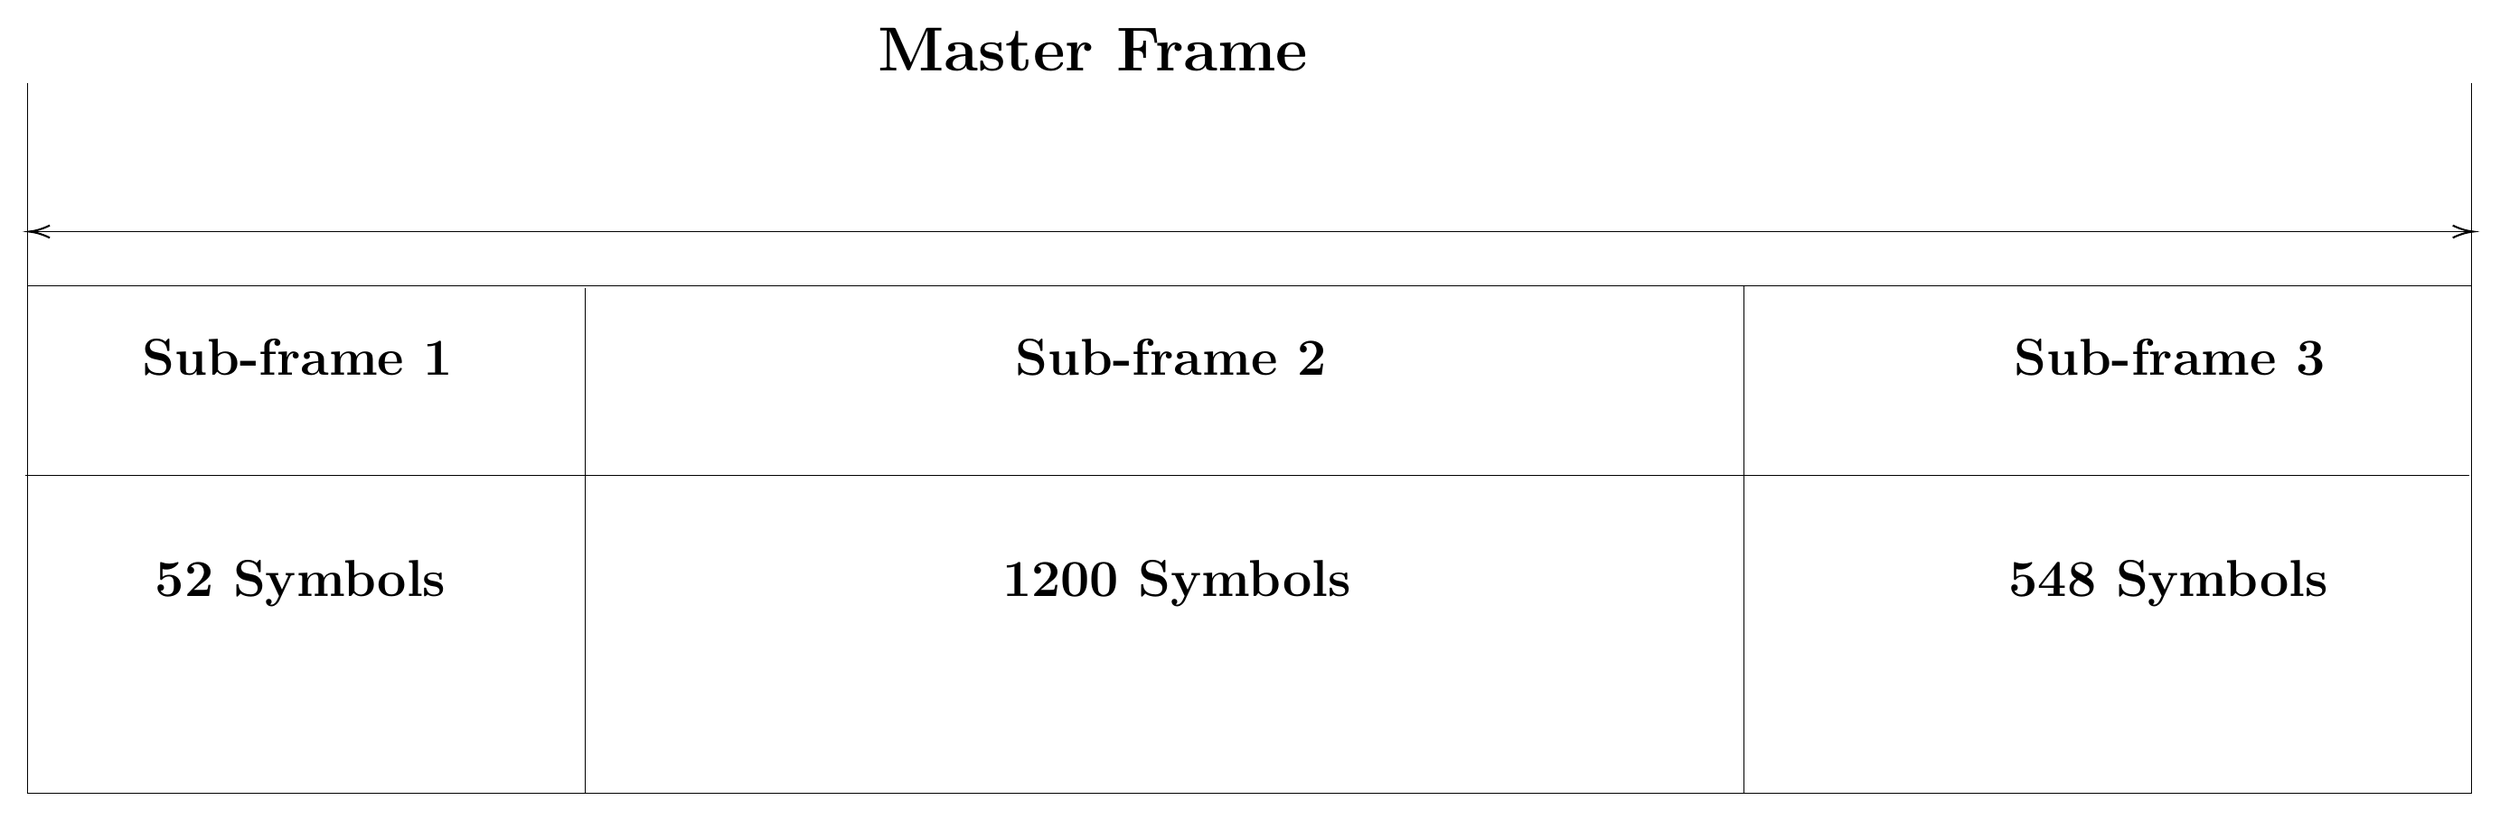
\begin{tikzpicture}[x=0.75pt,y=0.75pt,yscale=-1,xscale=1]
%uncomment if require: \path (0,300); %set diagram left start at 0, and has height of 300

%Shape: Rectangle [id:dp9371262813454737] 
\draw   (-282.77,4.09) -- (1020,4.09) -- (1020,274.5) -- (-282.77,274.5) -- cycle ;
%Straight Lines [id:da0083423994499785] 
\draw    (631.99,3.5) -- (631.99,23.44) -- (631.99,274.5) ;
%Straight Lines [id:da3433908286791536] 
\draw    (14.37,5.26) -- (14.37,274.5) ;
%Straight Lines [id:da03469922683437621] 
\draw    (-284,104.98) -- (-271.72,104.98) -- (1018.77,104.98) ;
%Straight Lines [id:da04694582378761214] 
\draw    (1020,4.09) -- (1020,-104.41) ;
%Straight Lines [id:da30228140719821583] 
\draw    (-282.77,4.09) -- (-282.77,-104.41) ;
%Straight Lines [id:da23260364134575484] 
\draw    (-280,-25.02) -- (1018.77,-25.02) ;
\draw [shift={(1020.77,-25.02)}, rotate = 180] [color={rgb, 255:red, 0; green, 0; blue, 0 }  ][line width=0.75]    (10.93,-3.29) .. controls (6.95,-1.4) and (3.31,-0.3) .. (0,0) .. controls (3.31,0.3) and (6.95,1.4) .. (10.93,3.29)   ;
\draw [shift={(-282,-25.02)}, rotate = 0] [color={rgb, 255:red, 0; green, 0; blue, 0 }  ][line width=0.75]    (10.93,-3.29) .. controls (6.95,-1.4) and (3.31,-0.3) .. (0,0) .. controls (3.31,0.3) and (6.95,1.4) .. (10.93,3.29)   ;

% Text Node
\draw (169.11,-135) node [anchor=north west][inner sep=0.75pt]   [align=left] {{\fontsize{3.33em}{4em}\selectfont \textbf{Master Frame}}};
% Text Node
\draw (775,31) node [anchor=north west][inner sep=0.75pt]   [align=left] {{\fontsize{2em}{2.4em}\selectfont \textbf{Sub-frame 3}}};
% Text Node
\draw (242.5,31) node [anchor=north west][inner sep=0.75pt]   [align=left] {{\fontsize{2em}{2.4em}\selectfont \textbf{Sub-frame 2}}};
% Text Node
\draw (-223,31) node [anchor=north west][inner sep=0.75pt]  [color={rgb, 255:red, 0; green, 0; blue, 0 }  ,opacity=1 ] [align=left] {{\fontsize{2em}{2.4em}\selectfont \textbf{Sub-frame 1}}};
% Text Node
\draw (235.5,149) node [anchor=north west][inner sep=0.75pt]   [align=left] {{\fontsize{2em}{2.4em}\selectfont \textbf{1200 Symbols}}};
% Text Node
\draw (-216,149) node [anchor=north west][inner sep=0.75pt]   [align=left] {{\fontsize{2em}{2.4em}\selectfont \textbf{52 Symbols}}};
% Text Node
\draw (772,149) node [anchor=north west][inner sep=0.75pt]   [align=left] {{\fontsize{2em}{2.4em}\selectfont \textbf{548 Symbols}}};


\end{tikzpicture}





   
\end{document}


